\documentclass[answers]{exam}
\usepackage{../../template}
\title{Assignment 1}
\author{niceguy}
\begin{document}
\maketitle

\begin{questions}

\question{A 10 GW$_e$ (Gigawatts electric power) fusion reactor operates at full power 80\% of the time for a year, at a 40\% thermal to electric efficiency, burning catalyzed D – D fuel (ie., 6 D $\rightarrow$ 2 H + 2 n + 2 $^4$He + 43.2 MeV). How many kg of deuterium will be consumed? How many cubic meters of ordinary water are needed to extract this much deuterium? Compare the energy released by fusion to that which would be released if the deuterium was used in a fuel cell to generate electricity.} \label{q1}

\begin{solution}
    Operating for 1 year, total energy produced to reach 10 GW is
    $$10 \times 10^9 \times 80\% \times (60 \times 60 \times 24 \times 365) \div 40\% = 6.31 \times 10^{17} \unit{J}$$
    Mass of deuterium (assuming molar mass of 2g) is
    $$6.31 \times 10^{17} \div \left(43.2 \times 1.60 \times 10^{-19} \times 10^6\right) \times 6 \times \frac{0.002}{6.02 \times 10^{23}} = 1820 \unit{kg}$$
    According to \url{https://www.iaea.org/newscenter/news/what-is-deuterium}, there are 33 grams of deuterium per cubic metre of seawater, so cubic metres needed is
    $$\frac{1820}{33 \times 10^{-3}} = 55100$$
    According to \url{https://rmi.org/run-on-less-with-hydrogen-fuel-cells}, hydrogen fuel cell efficiency is estimated to be 120 MJ/kg. Energy generated will then be
    $$1820 \times 120 \times 10^6 = 2.18 \times 10^{11} \unit{J}$$
    which is 6 orders of magnitude less.
\end{solution}

\question{A fusion reactor has a plasma of $T_i = T_e = 15$ keV and $n_i = n_e = 2 \times 10^{21} \unit{m^{-3}}$. What is the pressure in the reactor (in kPa, atm and tonnes/$\unit{m^2}$)? What part of the reactor must withstand this pressure? Compare the particle density with air at standard temperature and pressure. For a plasma volume of 50 $\unit{m^3}$, how much energy is contained in the plasma? If all of the fuel were to instantaneously fuse in D-T reactions ($n_D = n_T = \frac{n_i}{2}$), how much energy would be released (in ktons of TNT)? How much tritium is required? How much radioactivity (Bq, Ci) is associated with this much tritium? What is the value of this tritium (current price is ~ \$1 million per oz.)?}

\begin{solution}
    Assume that the ideal gas law holds. Then
    $$p = nkT = \frac{2}{3} n \left(\frac{3}{2}kT\right) = \frac{2}{3} En = \frac{2}{3} 15000 \times 1.6 \times 10^{-19} \times 2 \times 10^{21} = 3.2 \times 10^6 \unit{Pa}$$
    The reaction chamber must withstand this pressure. Particle density is $2\times10^{21}$, which is magnitudes lower than particle density of air, approximately $2.7 \times 10^{25}$. \\
    To find the energy in a given volume of plasma, we first rearrange the ideal gas law and substitute the expression for energy.
    \begin{align*}
        pV &= NkT \\
        \frac{3}{2} pV &= \frac{3}{2} NkT \\
        E &= \frac{3}{2} pV \\
          &= \frac{3}{2} 3.2 \times 10^6 \times 50 \\
          &= 240 \times 10^6 \unit{J}
    \end{align*}
    For D-T reactions, 17.6 MeV of energy is released per reaction. Energy released in total is then
    $$50 \times 2 \times 10^{21} \div 2 \times 17.6 \times 10^6 \times 1.6 \times 10^{-19} = 1.408 \times 10^{11}$$
    A kiloton of TNT is taken to be $4.184 \times 10^{12}\unit{J}$, so in terms of that, energy is
    $$1.408 \times 10^{11} \div 4.184 \times 10^{12} = 0.0337$$
    Tritium involved is
    $$50 \times 2 \times 10^{21} \div 2 \times \frac{3}{6.02 \times 10^{23}} = 0.249 \unit{g}$$
    Radioactivity of tritium is 9650 Ci per gram, so total radioactivity is
    $$9650 \times 0.249 = 2400\unit{Ci}$$
    1 ounce is 28.3 grams, so value is approximately
    $$0.249 \div 28.3 \times 10^6 = \$8800$$
\end{solution}

\question{Resources:}

\begin{parts}

\part{Is lithium a sufficient resource?}

\begin{solution}
    Volume of oceans is $1.37 \times 10^{18} \unit{m^3}$. This gives $1.37 \times 10^{18} \times 0.17 = 2.33 \times 10^{17}$ grams of lithium. Its molar mass is 6.941, so there are $2.33 \times 10^{17} \times \frac{6.02\times10^{23}}{6.941} = 2.02 \times 10^{40}$ moles of lithium. From the reaction, this translates to  $2.02 \times 10^{40} \times \frac{0.003}{6.02\times10^{23}} = 1.01 \times 10^{14}$ kilograms of tritium. This should be sufficient for some time, even if we don't use up our oceans.
\end{solution}

\part{How long will the deuterium in the oceans last?}

\begin{solution}
    We can solve this using information given Question \ref{q1}, and the internet (33 grams of deuterium per cubic metre of seawater). \\
    Number of molecules of deuterium in the ocean:
    $$1.37 \times 10^{18} \times 33 \times \frac{6.02\times10^{23}}{2} = 1.36 \times 10^{43}$$
    Energy generated in Joules is
    $$1.36 \times 10^{43} \times \frac{43.2 \times 10^6 \times 1.6 \times 10^{-19}}{6} = 1.57 \times 10^{31}$$
    Deuterium will then last (in years)
    $$1.57 \times 10^{31} \div 10^{21} = 1.57 \times 10^{10}$$
\end{solution}

\end{parts}

\question{Consider a terrestrial fusion device.}

\begin{parts}

\part{Find the energy produced per H that is fused.}

\begin{solution}
    Mass lost (in amu)
    $$1.00727644 \times 2 - 2.013553 - 0.0005485801 = 4.51 \times 10^{-4}$$
    Energy is then
    $$E = mc^2 = 4.51 \times \frac{0.001}{6.02\times10^{23}} \times (3 \times 10^8)^2 = 6.75 \times 10^{-14} \unit{J} = 0.422 \unit{MeV}$$
\end{solution}

\part{What mass and volume of material would be required? Conclusions?}

\begin{solution}
    Adding up the reactions, 6H is converted to $^4$He, $^2$H, and $2e^+$. Mass lost (in amu) is
    $$1.00727644 \times 6 - 4.001503 - 2.013553 - 0.0005485801 \times 2 = 0.0275$$
    Energy per reaction is then
    $$E = mc^2 = \frac{0.0275}{6.02\times10^{23}} \times (3\times10^8)^2 = 4.11 \times 10^{-9}\unit{J}$$
    Power is then
    $$P = \frac{En}{t}$$
    where $n$ is the number of the 6H atoms needed for each reaction, and $t$ is the expected time per reaction. Then
    \begin{align*}
        9\times10^9 &= \frac{4.11 \times 10^{-9}n}{2\times7\times10^9\times(60 \times 60 \times 24 \times 365)} \\
        n &= 9.67 \times 10^{35} \\
          &= 1.61 \times 10^{12} \unit{mol} \\
          &= 9.64 \times 10^9\unit{kg} \\
          &= 1.15 \times 10^{11} \unit{m^3}
    \end{align*}
    This is probably unsustainable, because a large amount of hydrogen gas is needed.
\end{solution}

\part{Estimate how long the sun will continue to shine.}

\begin{solution}
    This is a tricky question. Technically, one could argue the sun would still be shining as long as there are a handful of hydrogen atoms left. This could take a very long time, depending on the distribution of reaction time. Therefore, we assume by the time mean time passes, the sun will essentially stop shining. The sun has been here for 4.6 billion years, so it will still shine for $7-4.6=2.4$ billion years. Note that the mean time needed for the second and third reactions are negligible.
\end{solution}

\end{parts}

\question{}

\begin{parts}

\part{Find the required particle energy and comment on the implications.}

\begin{solution}
    Normally, kinetic energy on the order of 100 keV is needed. If the Coulomb barrier has to be overcome without tunneling, energy needed is
    $$E = k\frac{q_1q_2}{r} = 4.60 \times 10^{-13} Z_1Z_2 \unit{J} = 288 Z_1Z_2 \unit{keV}$$
    Particle energy needed is then \\
    \begin{tabular}{c c}
            \hline
            Fusion Reaction & Energy (keV) \\
            \hline
            DT & 288 \\
            \hline
            DDn & 288 \\
            \hline
            DDp & 288 \\
            \hline
            TT & 288 \\
            \hline
            D-$^3$He & 575 \\
            \hline
            p-$^6$Li & 863 \\
            \hline
            p-$^{11}$B & 1440 \\
            \hline
    \end{tabular} \\
    For DT fusion with tunneling, energy needed is to the order of 10 keV, which is one order of magnitude lower. Hence quantum tunneling is essential for fusion to work.
\end{solution}

\part{For the DT reaction, compare the behaviour with Dolan.}

\begin{solution}
    From Dolan, we have $\sigma(50\unit{keV}) = 1.6 \times 10^{-28}\unit{m^2}$. However, here we find energy using the reduced mass, but in Dolan the energy of the deuterium is used instead. Now
    $$E = \frac{1}{2}Mv^2 = \frac{1}{2}m_Dv^2 \times \frac{M}{m_D} = \frac{E_DM}{m_D}$$
    Simplifying the expression with D-T values, we have
    \begin{align*}
        \sigma &= \frac{C}{E_D} \times \frac{m_D}{M} \exp\left(-\frac{\pi M^{1/2}m_D^{1/2}q_1q_2}{\sqrt{2}\varepsilon_0hE_D^{1/2}M^{1/2}}\right) \\
               &= \frac{C}{E_D} \times \frac{m_D}{M} \exp\left(-\frac{\pi m_D^{1/2}q_1q_2}{\sqrt{2}\varepsilon_0hE_D^{1/2}}\right)\\
    \end{align*}
    Mass of deuterium is $3.34\times10^{-27}\unit{kg}$. The reduced mass is
    $$M = \frac{m_1m_2}{m_1+m_2} = \frac{3.34\times10^{-27}\times5.01\times10^{-27}}{3.34\times10^{-27}+5.01\times10^{-27}} = 2.00 \times 10^{-27}$$
    This gives
    $$\sigma(E_D) = \frac{1.67C}{E_D}\exp\left(-\frac{5.60\times10^{-7}}{E_D^{1/2}}\right)$$
    Substituting $E_D = 50\unit{keV}$ and $\sigma = 1.6\times10^{-28}\unit{m^2}$, we have
    $$C = 4.03 \times 10^{-40}$$
    Plotting, we have \\
    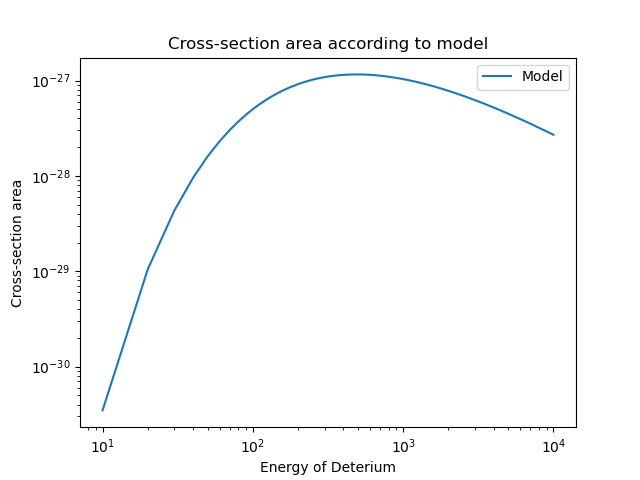
\includegraphics[width=\textwidth]{model.png}
    The figure in Dolan is \\
    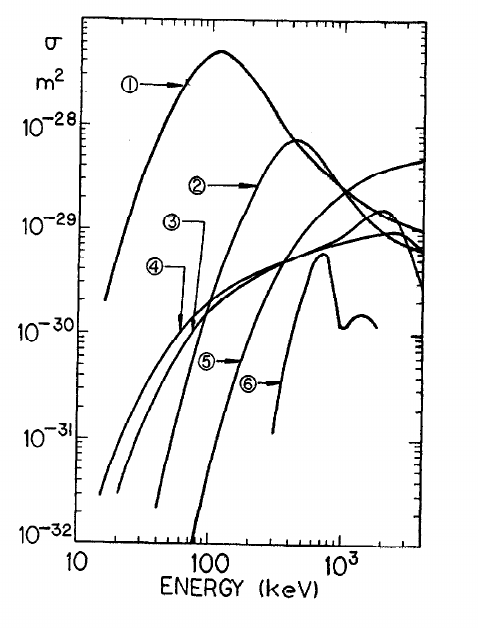
\includegraphics[width=\textwidth]{2c1.png}
    Both agree up until $\sigma(E)$ reaches its maximum. Afterwards, the model overestimates the cross section. In class, we discussed how cross section decreases at higher temperatures, since particles don't "stay still" long enough for reactions to occur. This may not be accounted for in the model, which explains its deviation.
\end{solution}

\end{parts}

\question{What was the first tokamak operating outside the Soviet Union?}

\begin{solution}
    Symmetric Tokamak.
\end{solution}

\end{questions}
\end{document}
